\documentclass[border=4pt]{standalone}
\usepackage{amsmath,amssymb,tikz}
\usetikzlibrary{arrows.meta,calc}
\definecolor{figB}{RGB}{31,90,166}\definecolor{figR}{RGB}{176,48,48}\definecolor{figG}{RGB}{46,125,50}\definecolor{figO}{RGB}{214,120,20}
\begin{document}
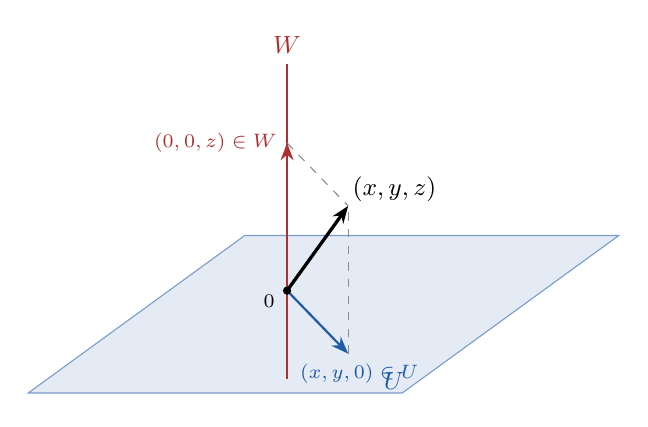
\begin{tikzpicture}[scale=1.25,>={Stealth[length=2.2mm]},x={(-0.55cm,-0.4cm)},y={(1cm,0cm)},z={(0cm,1cm)}]
\fill[figB!12] (-1.4,-1.2,0)--(2.6,-1.2,0)--(2.6,2.6,0)--(-1.4,2.6,0)--cycle;
\draw[figB!60] (-1.4,-1.2,0)--(2.6,-1.2,0)--(2.6,2.6,0)--(-1.4,2.6,0)--cycle;
\node[figB,font=\small] at (2.3,2.35,0) {$U$};
\draw[figR,thick] (0,0,-0.9)--(0,0,0);
\draw[figR,thick] (0,0,0)--(0,0,2.3) node[above,font=\small]{$W$};
\coordinate (O) at (0,0,0); \coordinate (P) at (1.6,1.5,0); \coordinate (V) at (1.6,1.5,1.5);
\draw[black!45,dashed] (P)--(V);
\draw[black!45,dashed] (0,0,1.5)--(V);
\draw[->,thick,figB] (O)--(P) node[below,font=\scriptsize,xshift=4pt]{$(x,y,0)\in U$};
\draw[->,thick,figR] (O)--(0,0,1.5) node[left,font=\scriptsize]{$(0,0,z)\in W$};
\draw[->,very thick] (O)--(V) node[above right,font=\small,inner sep=1pt]{$(x,y,z)$};
\fill (O) circle (1.2pt) node[left,font=\scriptsize,xshift=-1pt,yshift=-4pt]{$0$};
\end{tikzpicture}
\end{document}
